%!Mode::"UTF-8"
\documentclass[12pt]{article}

% 页面设置
\usepackage{geometry}
\geometry{left=2.5cm, right=2.5cm, top=2.5cm, bottom=2.5cm}
\usepackage{graphicx}
\usepackage{ctex}
\usepackage{fontspec}
\usepackage{setspace}

% 代码设置
\usepackage{listings}
\usepackage{color}
\setmonofont{Consolas}
\definecolor{listing}{gray}{0.97}
\lstset{
	backgroundcolor=\color{listing},
	basicstyle=\footnotesize,
	numbers=left,
	numberstyle=\footnotesize,
	stepnumber=1,
	aboveskip={0.5\baselineskip},
	belowskip={0.5\baselineskip},
	columns=fullflexible,
	breaklines=true,
	breakatwhitespace=true,
	frame=single,
	basicstyle=\ttfamily,
	numberstyle=\ttfamily,
	tabsize=2
}

% 字体设置
\setmainfont{Times New Roman}
\setCJKmainfont{SimSun}
\setCJKsansfont{SimHei}

% 表格设置
\usepackage{makecell}
\newcommand{\addcell}[2][4]{\makecell{\zihao{#1}\textsf{#2}}}
\usepackage{titlesec}
\usepackage{booktabs}
\usepackage{tabularx}

% 设置图注、表注
\usepackage{caption}
\usepackage{bicaption}
\captionsetup{labelsep=quad, font={small, bf}, skip=2pt}
\DeclareCaptionOption{english}[]{
    \renewcommand\figurename{Fig.}
    \renewcommand\tablename{Table}
}
\captionsetup[bi-second]{english}

% 设置页眉
\usepackage{fancyhdr}
\pagestyle{fancy}
\fancypagestyle{preContent}{
    \fancyhead[L]{\zihao{-5} 物理化学实验}
    \fancyhead[C]{\zihao{-5} 实验十二\ \ 分子动力学模拟}
    \fancyhead[R]{\zihao{-5} 1800011828\ 王宇哲}
}
\pagestyle{preContent}

%	设置首页页眉页脚
\fancypagestyle{plain}{
	\fancyhead[L]{\zihao{-5} 物理化学实验}
	\fancyhead[C]{\zihao{-5} 实验十二\ \ 分子动力学模拟}
	\fancyhead[R]{\zihao{-5} 1800011828\ 王宇哲}
	\cfoot{}
}

% 设置标题格式
\titleformat*{\section}{\zihao{4}\sffamily}
\titleformat*{\subsection}{\zihao{-4}\sffamily}
\titleformat*{\subsubsection}{\zihao{-4}\sffamily}
\titlespacing*{\section}{0pt}{10pt}{10pt}
\titlespacing*{\subsection}{0pt}{10pt}{5pt}
\titlespacing*{\subsubsection}{0pt}{10pt}{5pt}

% 设置引用格式
\usepackage[super,round,comma,compress]{natbib}

\usepackage{amsmath}
\usepackage{amssymb}

%设置封面
\begin{document}
    % 标题页
    \begin{titlepage}
    	% 页眉
    	\thispagestyle{plain}
        % 图片
        \begin{figure}[h]
            \centering
            \includegraphics{pku.png}
        \end{figure}
        \vspace{24pt}
        % 标题
        \centerline{\zihao{-0} \textsf{物理化学实验报告}}
        \vspace{40pt} % 空行
        \begin{center}
            \begin{tabular}{cp{8.5cm}}
                % 题目
                \addcell[2]{题目:\ } & \addcell[2]{分子动力学模拟} \\
                \cline{2-2}
            \end{tabular}
        \end{center}
        \vspace{20pt} % 空行
        \begin{center}
            \doublespacing
            \begin{tabular}{cp{5cm}}
                % 姓名
                \addcell{姓\phantom{空格}名:\ } & \addcell{王宇哲} \\
                \cline{2-2}
                % 学号
                \addcell{学\phantom{空格}号:\ } & \addcell{1800011828}\\
                \cline{2-2}
                % 组别
                \addcell{组\phantom{空格}别:\ } & \addcell{11组} \\
                \cline{2-2}
                % 实验日期
                \addcell{实验日期:\ } & \addcell{2020.10.14}\\
                \cline{2-2}
                % 室温
                \addcell{室\phantom{空格}温:\ } & \addcell{291.75\ K}\\
                \cline{2-2}
                % 大气压强
                \addcell{大气压强:\ } & \addcell{102.62\ kPa}\\
                \cline{2-2}
            \end{tabular}
            \begin{tabular*}{\textwidth}{c}
                \\ % 这是空行
                \\ % 这是空行
                \\ % 这是空行
                \\ % 这是空行
                \hline % 分割线
            \end{tabular*}
        \end{center}
        % 摘要
        \textsf{摘\ \ 要}\ \ 本实验通过分子动力学模拟方法,使用AMBER 14软件构建了丙氨酸12肽链结构,对初始结构进行了结构优化,对优化后结构进行了加热升温模拟和折叠模拟,使用VMD软件观察优化后结构、加热后终态构象、折叠过程模拟轨迹,分析数据得到了折叠过程最低势能结构,从而初步了解了分子动力学模拟的基本原理和方法。
        \\
        \\
        % 关键字
        \textsf{关键词}\ \ 分子动力学模拟;丙氨酸12肽链;AMBER 14
    \end{titlepage}

    \section{引言}
	略
               
\vbox{}        
    \section{实验部分}
    	\subsection{软件程序}
    	AMBER 14软件、VMD软件,在Ubuntu系统上运行。
    	
    	 \subsection{实验内容\citealp{physchemlab}}
			\subsubsection{初始结构的构建}
			使用tleap的sequence命令构建初始结构。在桌面建立姓名首字母文件夹wyz,进入文件夹后,在终端执行命令
\begin{lstlisting}
	tleap -f $AMBERHOME/dat/leap/cmd/leaprc.ff14SB
\end{lstlisting}
以调用力场文件leaprc.ff14SB;在运行tleap后出现的提示符下键入
\begin{lstlisting}
	>ala12=sequence {NALA ALA ALA ALA ALA ALA ALA ALA ALA ALA ALA CALA}
	>saveamberparm ala12 ala12.prmtop ala12.inpcrd
	>quit
\end{lstlisting}
从而构建丙氨酸12肽链初始结构,并在wyz文件夹中生成文件ala12.prmtop及ala12.inpcrd。
	
	
			\subsubsection{结构优化}
		在wyz文件夹中创建文件min.in。在终端执行命令
		\begin{lstlisting}
	vim min.in
		\end{lstlisting}
		向min.in文件中写入
		\begin{lstlisting}
	Stage 1 - minimisation of ALA12
	&cntrl
	imin=1, maxcyc=1000, ncyc=500, cut=999., rgbmax=999., igb=1, ntb=0, ntpr=100
	/
		\end{lstlisting}
		在终端执行命令
\begin{lstlisting}
	mpirun –np 4 sander.MPI –O –i min.in –p ala12.prmtop –c ala12.inpcrd –o ala12_min.out –r ala12_min.rst7
\end{lstlisting}
	以进行结构优化,在wyz文件夹中生成文件ala12.inpcrd、ala12\_min.out及ala12\_min.rst7。在终端执行命令
\begin{lstlisting}
	vmd
\end{lstlisting}
	以打开VMD程序,载入文件ala12.prmtop,随后载入初始结构文件ala12.inpcrd及结构优化后的结构文件ala12\_min.rst7,在VMD程序可视化窗口中进行对比。
	
	
	
			\subsubsection{加热升温至300 K}
			在wyz文件夹中创建文件heat.in。在终端执行命令
	\begin{lstlisting}
	vim heat.in
\end{lstlisting}
向heat.in文件中写入
\begin{lstlisting}
	Stage 2 heating of ALA12 0 to 300K
	&cntrl
	imin=0, irest=0, ntx=1,
	nstlim=20000, dt=0.001, ntc=1, ntf=1, ntt=3, gamma_ln=1.0, ig=-1, tempi=0.0, temp0=300.0, ntpr=100, ntwx=100, ntb=0, igb=1, cut=999., rgbmax=999., ioutfm=1
	/
\end{lstlisting}
在终端执行命令
\begin{lstlisting}
	mpirun –np 4 sander.MPI –O –i heat.in –p ala12.prmtop –c ala12_min.rst7 –o ala12_heat.out –r ala12_heat.rst7 –x ala12_heat.nc
\end{lstlisting}
模拟分子加热升温至300 K,在wyz文件夹中生成输出文件ala12\_heat.out、ala12\_heat.rst7及ala12\_heat.nc。打开VMD程序,载入文件ala12.prmtop,随后载入加热升温至300 K后的结构文件ala12\_heat.rst7,以“new ribbons”和“lines”表示丙氨酸12肽链加热至300 K的终态构象。\par
处理得到的输出文件。在终端执行命令
\begin{lstlisting}
	process_mdout.perl ala12_heat.out
\end{lstlisting}
在wyz文件夹中生成一系列以summary开头的输出文件,包括有关温度的summary.TEMP、有关动能的summary.EKTOT及有关势能的summary.EPTOT。作出系统温度、动能及势能随时间变化的曲线。
			\subsubsection{折叠模拟}
在wyz文件夹中创建文件md.in。在终端执行命令
\begin{lstlisting}
	vim md.in
\end{lstlisting}
向md.in文件中写入
\begin{lstlisting}
	Stage 3 production run of ALA12 at 300K
	&cntrl
	imin=0, irest=1, ntx=5, nstlim=500000, dt=0.002, ntc=2, ntf=2, ntt=3, gamma_ln=1.0, ig=-1, tempi=300.0, temp0=300.0, ntpr=500, ntwx=500, ntb=0, igb=1, cut=999., rgbmax=999., ioutfm=1
	/
\end{lstlisting}
在终端执行命令
\begin{lstlisting}
	mpirun –np 4 sander.MPI –O –i md.in –p ala12.prmtop –c ala12_heat.rst7 –o ala12_md1.out –r ala12_md1.rst7 –x ala12_md1.nc
\end{lstlisting}
以进行折叠模拟,在wyz文件夹中生成输出文件ala12\_md1.out、ala12\_md1.rst7及ala12\_md1.nc。打开VMD程序,载入文件ala12.prmtop,随后载入第1次折叠模拟的轨迹文件ala12\_md1.nc,以“new cartoon”表示画出分子结构,观察分子结构变化及丙氨酸12肽链是否形成$\alpha$-螺旋。\par
实验中,第1次折叠模拟未形成$\alpha$-螺旋;以ala12\_md1.rst7作为输入文件,继续进行第2次折叠模拟。在终端执行命令
\begin{lstlisting}
	mpirun –np 4 sander.MPI –O –i md.in –p ala12.prmtop –c ala12_md1.rst7 –o ala12_md2.out –r ala12_md2.rst7 –x ala12_md2.nc
\end{lstlisting}
在wyz文件夹中生成输出文件ala12\_md2.out、ala12\_md2.rst7及ala12\_md2.nc。依此过程重复进行,共重复4次,第4次折叠模拟后观察到丙氨酸12肽链形成$\alpha$-螺旋,结束折叠模拟。\par
整理wyz文件夹中的输出文件。在wyz文件夹中建立子文件夹md1、md2、md3、md4,分别把ala12\_md1.out、ala12\_md2.out、ala12\_md3.out、ala12\_md4.out
复制进4个文件夹。
			\subsubsection{结果分析}
处理输出文件,找到最低势能结构。进入wyz文件夹的子文件夹md1,在终端执行命令
\begin{lstlisting}
	process_mdout.perl ala12_md1.out
\end{lstlisting}
得到势能文件summary.EPTOT。\par
对折叠模拟过程的势能按从小到大排序。在终端执行命令
\begin{lstlisting}
	sort -k 2 -n summary.EPTOT|head-10
\end{lstlisting}
记录输出结果第一行的势能。\par
在子文件夹md1、md2、md3、md4中分别进行上述操作,比较各势能大小,发现最低势能$-74.9130\ \ \rm kcal \cdot mol^{-1}$对应第4次折叠模拟的$539$帧;打开VMD程序,载入文件ala12.prmtop,随后载入第4次折叠模拟的轨迹文件ala12\_md4.nc,找到第$539$帧对应的最低能量结构。\par
根据4次折叠模拟生成的4个势能文件summary.EPTOT的数据,作出系统势能随时间变化的曲线。\par
计算折叠模拟过程的RMSD。打开VMD程序,载入文件ala12.prmtop,随后载入4次折叠模拟的轨迹文件ala12\_md1.nc、ala12\_md2.nc、ala12\_md3.nc及ala12\_md4.nc;在VMD中打开RMSD Trajectory Tool窗口,设置相关参数,点击ALIGN进行校正后,点击RMSD,计算每一帧相对于参考帧的RMSD,输出结果文件trajrmsd.dat;作出折叠模拟过程中RMSD随时间的变化。
\vbox{}  
	 \section{数据与结果}
 		\subsection{实验数据记录及处理}
 		            \subsubsection{初始结构的构建与结构优化}
打开VMD程序,载入初始结构文件ala12.inpcrd及结构优化后的结构文件ala12\_min.rst7,在VMD程序可视化窗口中用lines形式重叠显示初始结构和优化后的结构,如\textbf{图1}所示。
 		 \begin{figure}[h]
 			\centering
 			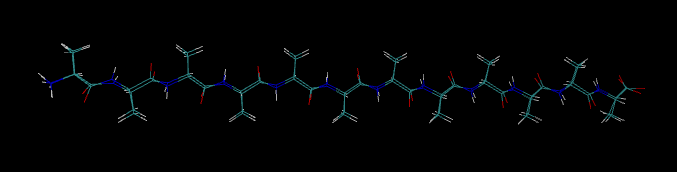
\includegraphics[width=0.7\textwidth]{1.png}
 			\bicaption{丙氨酸12肽链的初始结构与优化结构对比}{Comparison of initial structure and optimized structure of alanine 12 peptide chain}
 		\end{figure}
\par
对比两个结构可以发现,初始结构与优化后的结构整体高度相似,丙氨酸12肽链的主链构象基本未发生改变,仅有部分支链的键角发生了变化。
 	

 	\subsubsection{加热升温至300 K}
打开VMD程序,载入丙氨酸12肽链模拟加热升温至300 K后的结构文件ala12\_heat.rst,在VMD程序可视化窗口中显示加热后的终态构象,分别用new ribbons形式示于\textbf{图2}、用lines形式示于\textbf{图3}。

\begin{figure}[h]
	\centering
	
\includegraphics[width=0.7\textwidth]{new.png}
	\bicaption{New ribbons形式表示的丙氨酸12肽链加热升温至300 K的结构}{The structure of alanine 12 peptide chain heated to 300 K in the form of new ribbons}
\end{figure}

 \begin{figure}[h]
	\centering
	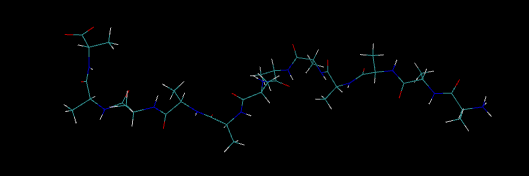
\includegraphics[width=0.7\textwidth]{lines.png}
	\bicaption{Liness形式表示的丙氨酸12肽链加热升温至300 K的结构}{The structure of alanine 12 peptide chain heated to 300 K in the form of lines}
\end{figure}
\par
读取丙氨酸12肽链模拟加热升温至300 K过程的温度、动能、势能文件summary.TEMP、summary.EKTOT、summary.EPTOT,用python matplotlib包作出系统温度、动能、势能随时间变化的曲线。\par
作出系统温度随时间变化的曲线如\textbf{图4}所示。根据\textbf{图4}可以看出,系统温度由0 K迅速上升,经过约5.0 ps即升温至300 K,随后在300 K附近上下波动;
\begin{figure}[h]
	\centering
	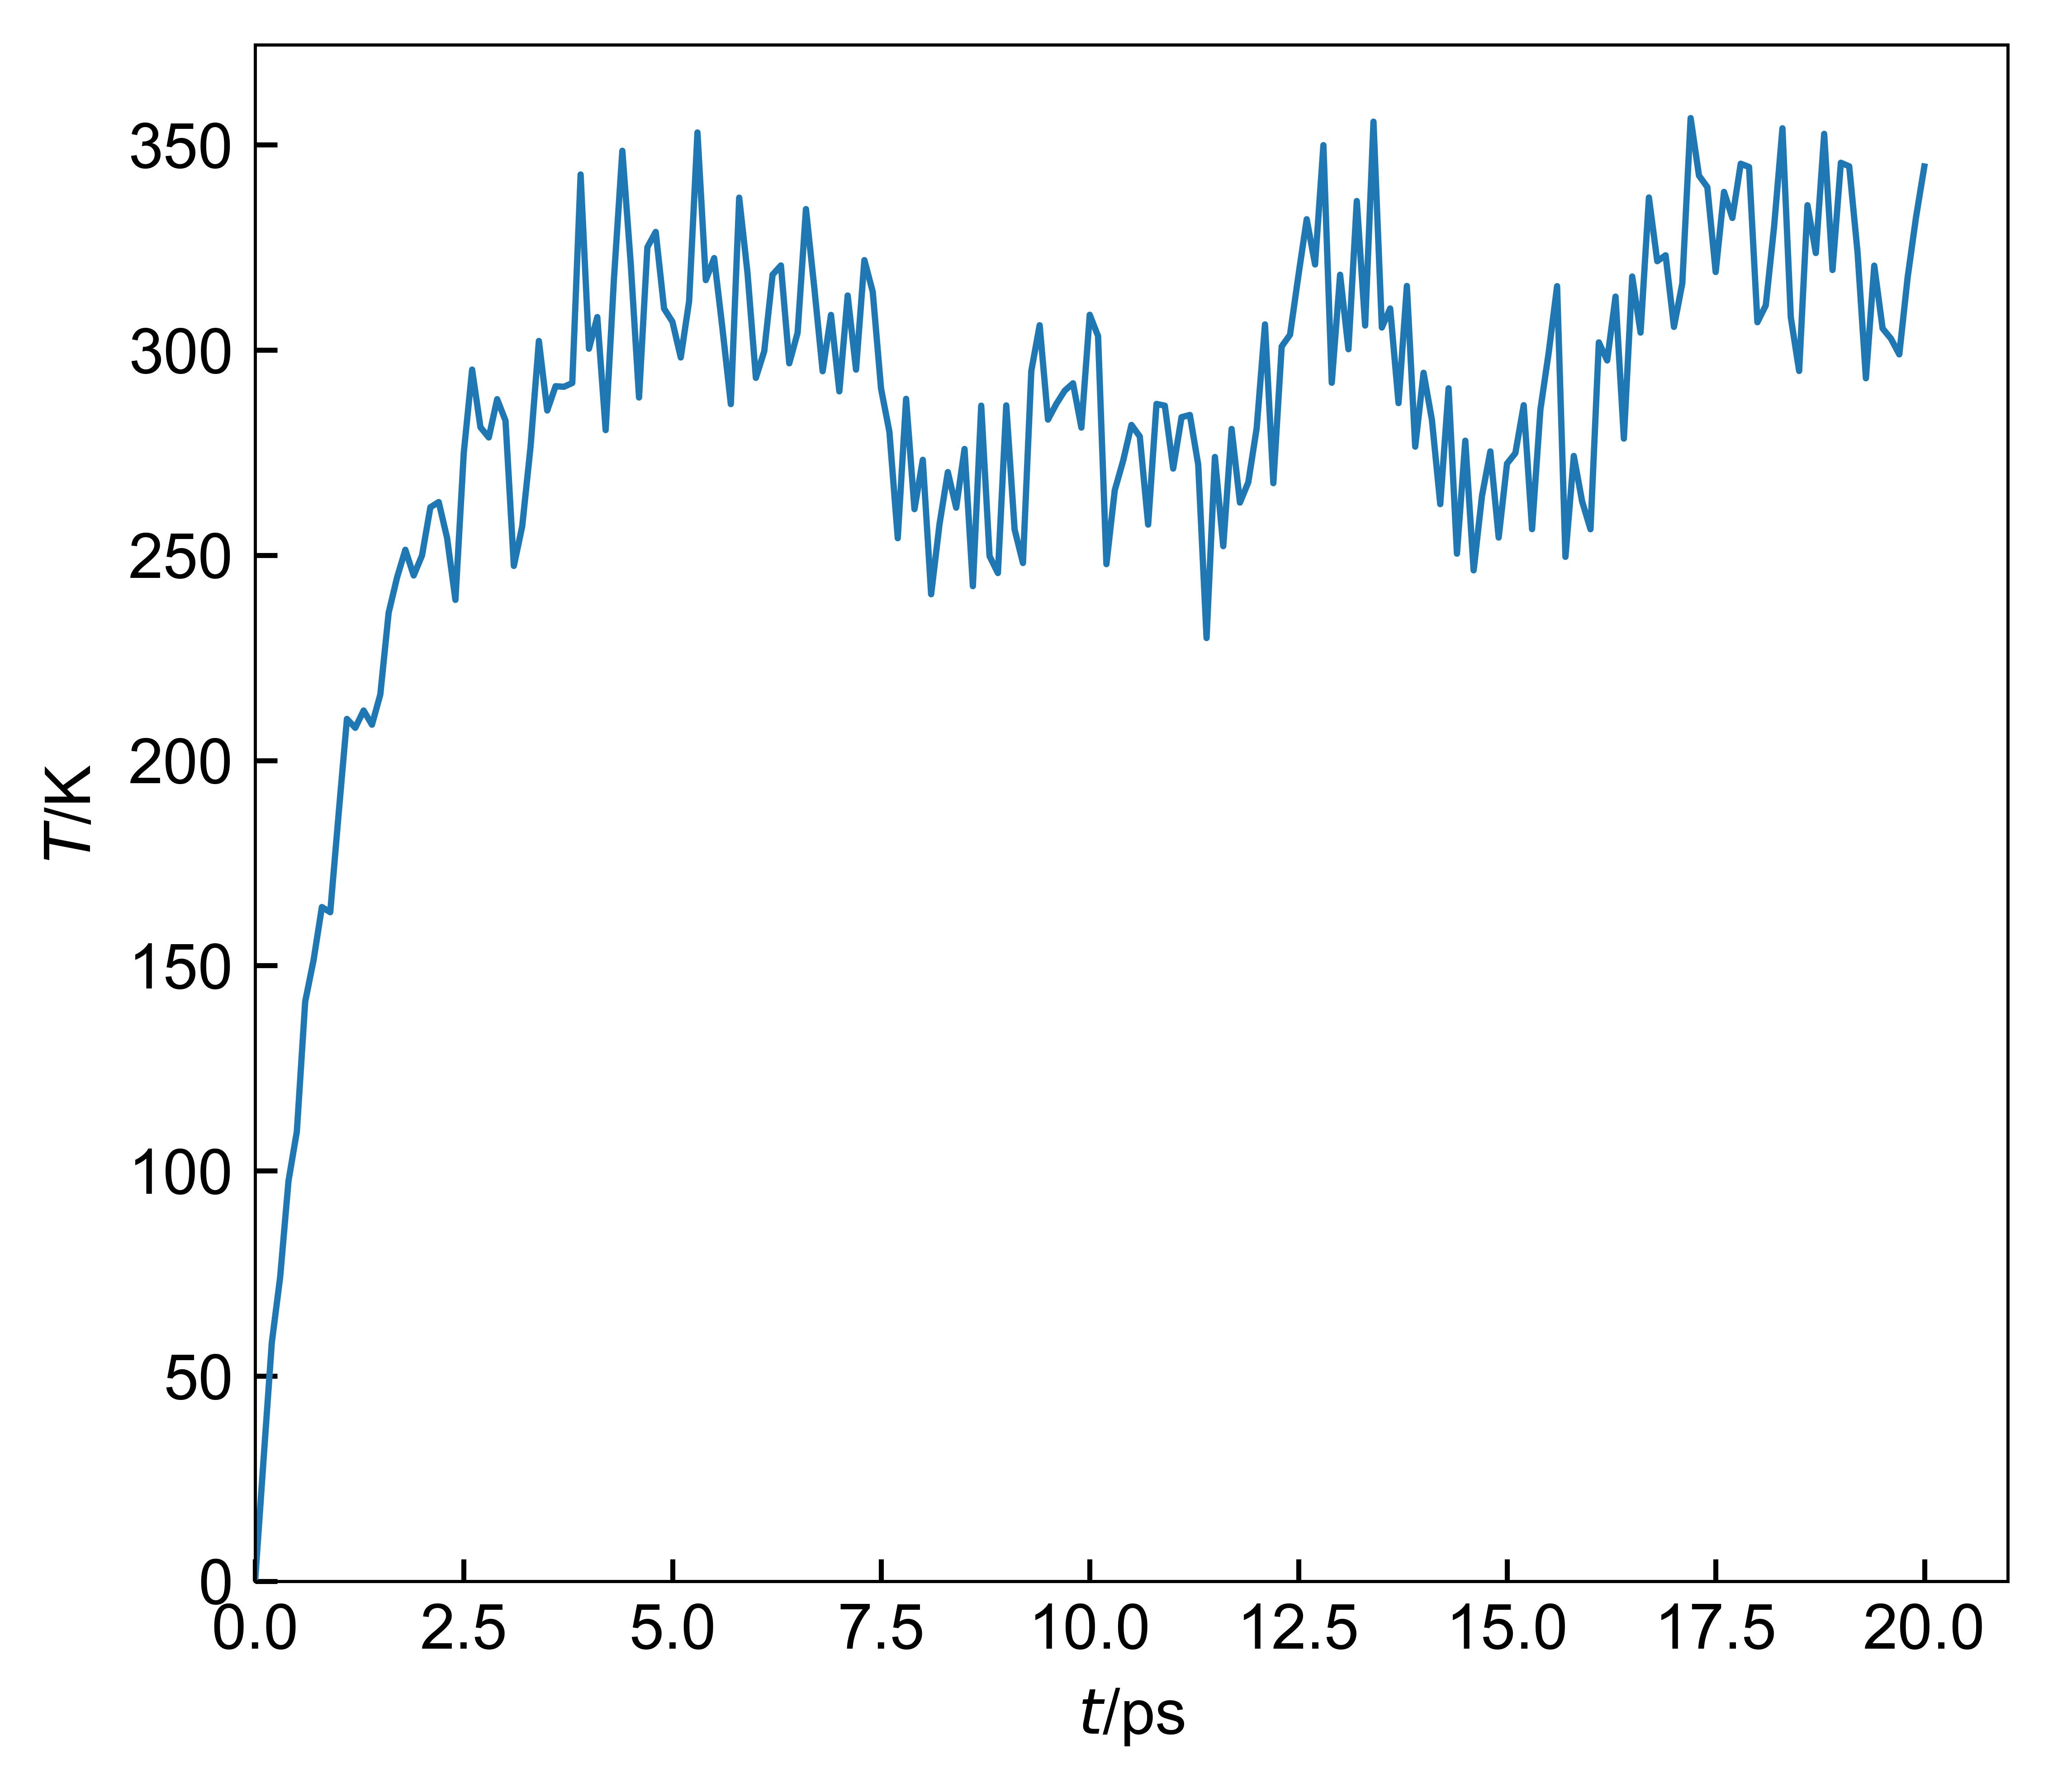
\includegraphics[width=0.5\textwidth]{temp.jpg}
	\bicaption{丙氨酸12肽链加热升温至300 K体系温度随时间的变化}{System temperature change of alanine 12 peptide chain heated to 300 K}
\end{figure}
\par
作出系统动能随时间变化的曲线如\textbf{图5}所示;作图前,通过单位换算
$$ 1\ \ {\rm kJ \cdot kcal^{-1}}=4.18585 \ \ {\rm kJ \cdot mol^{-1}} $$
已将能量换算为以${\rm kJ \cdot mol^{-1}}$为单位,下同;根据\textbf{图5}可以看出,系统动能由0迅速上升,同样经过约5.0 ps达到相对稳定,随后在$450 \ \ {\rm kJ \cdot mol^{-1}}$附近上下波动;
\begin{figure}[h]
	\centering
	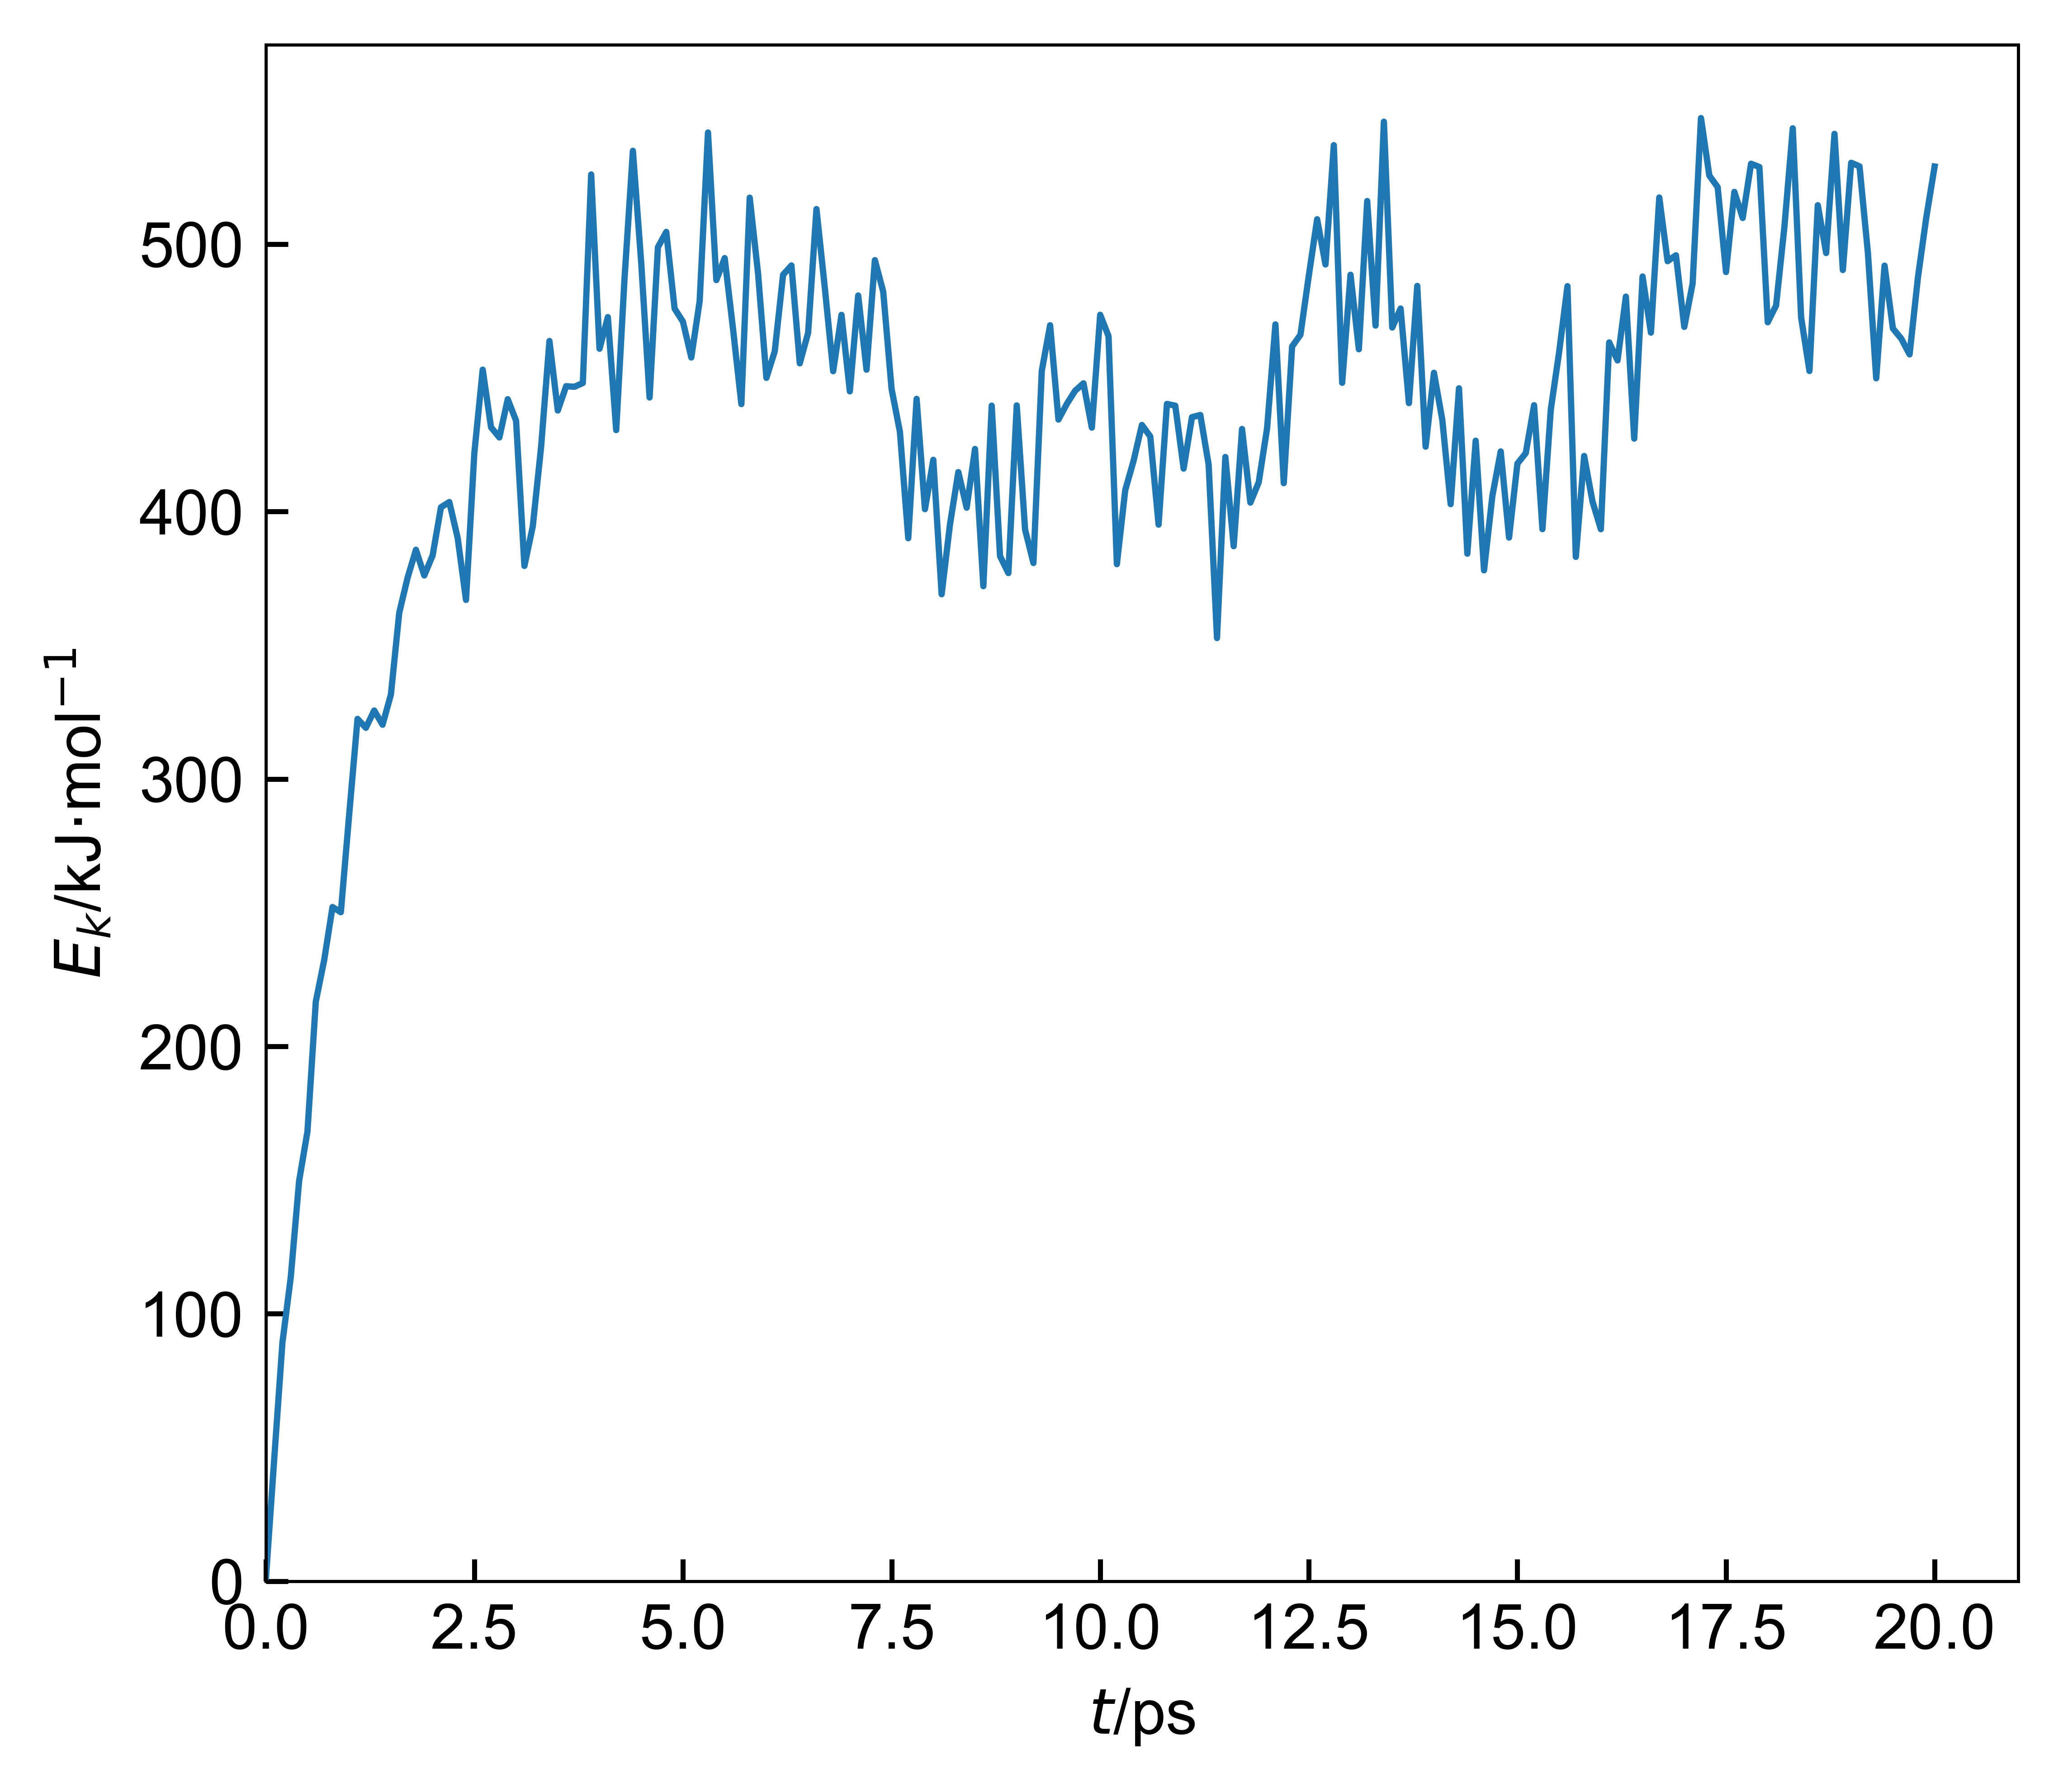
\includegraphics[width=0.5\textwidth]{ektot.jpg}
	\bicaption{丙氨酸12肽链加热升温至300 K体系动能随时间的变化}{System kinetic energy change of alanine 12 peptide chain heated to 300 K}
\end{figure}
\par
作出系统势能随时间变化的曲线如\textbf{图6}所示;根据\textbf{图6}可以看出,系统势能迅速上升,同样经过约5.0 ps达到相对稳定,随后在$-100 \ \ {\rm kJ \cdot mol^{-1}}$附近上下波动。
\begin{figure}[h]
	\centering
	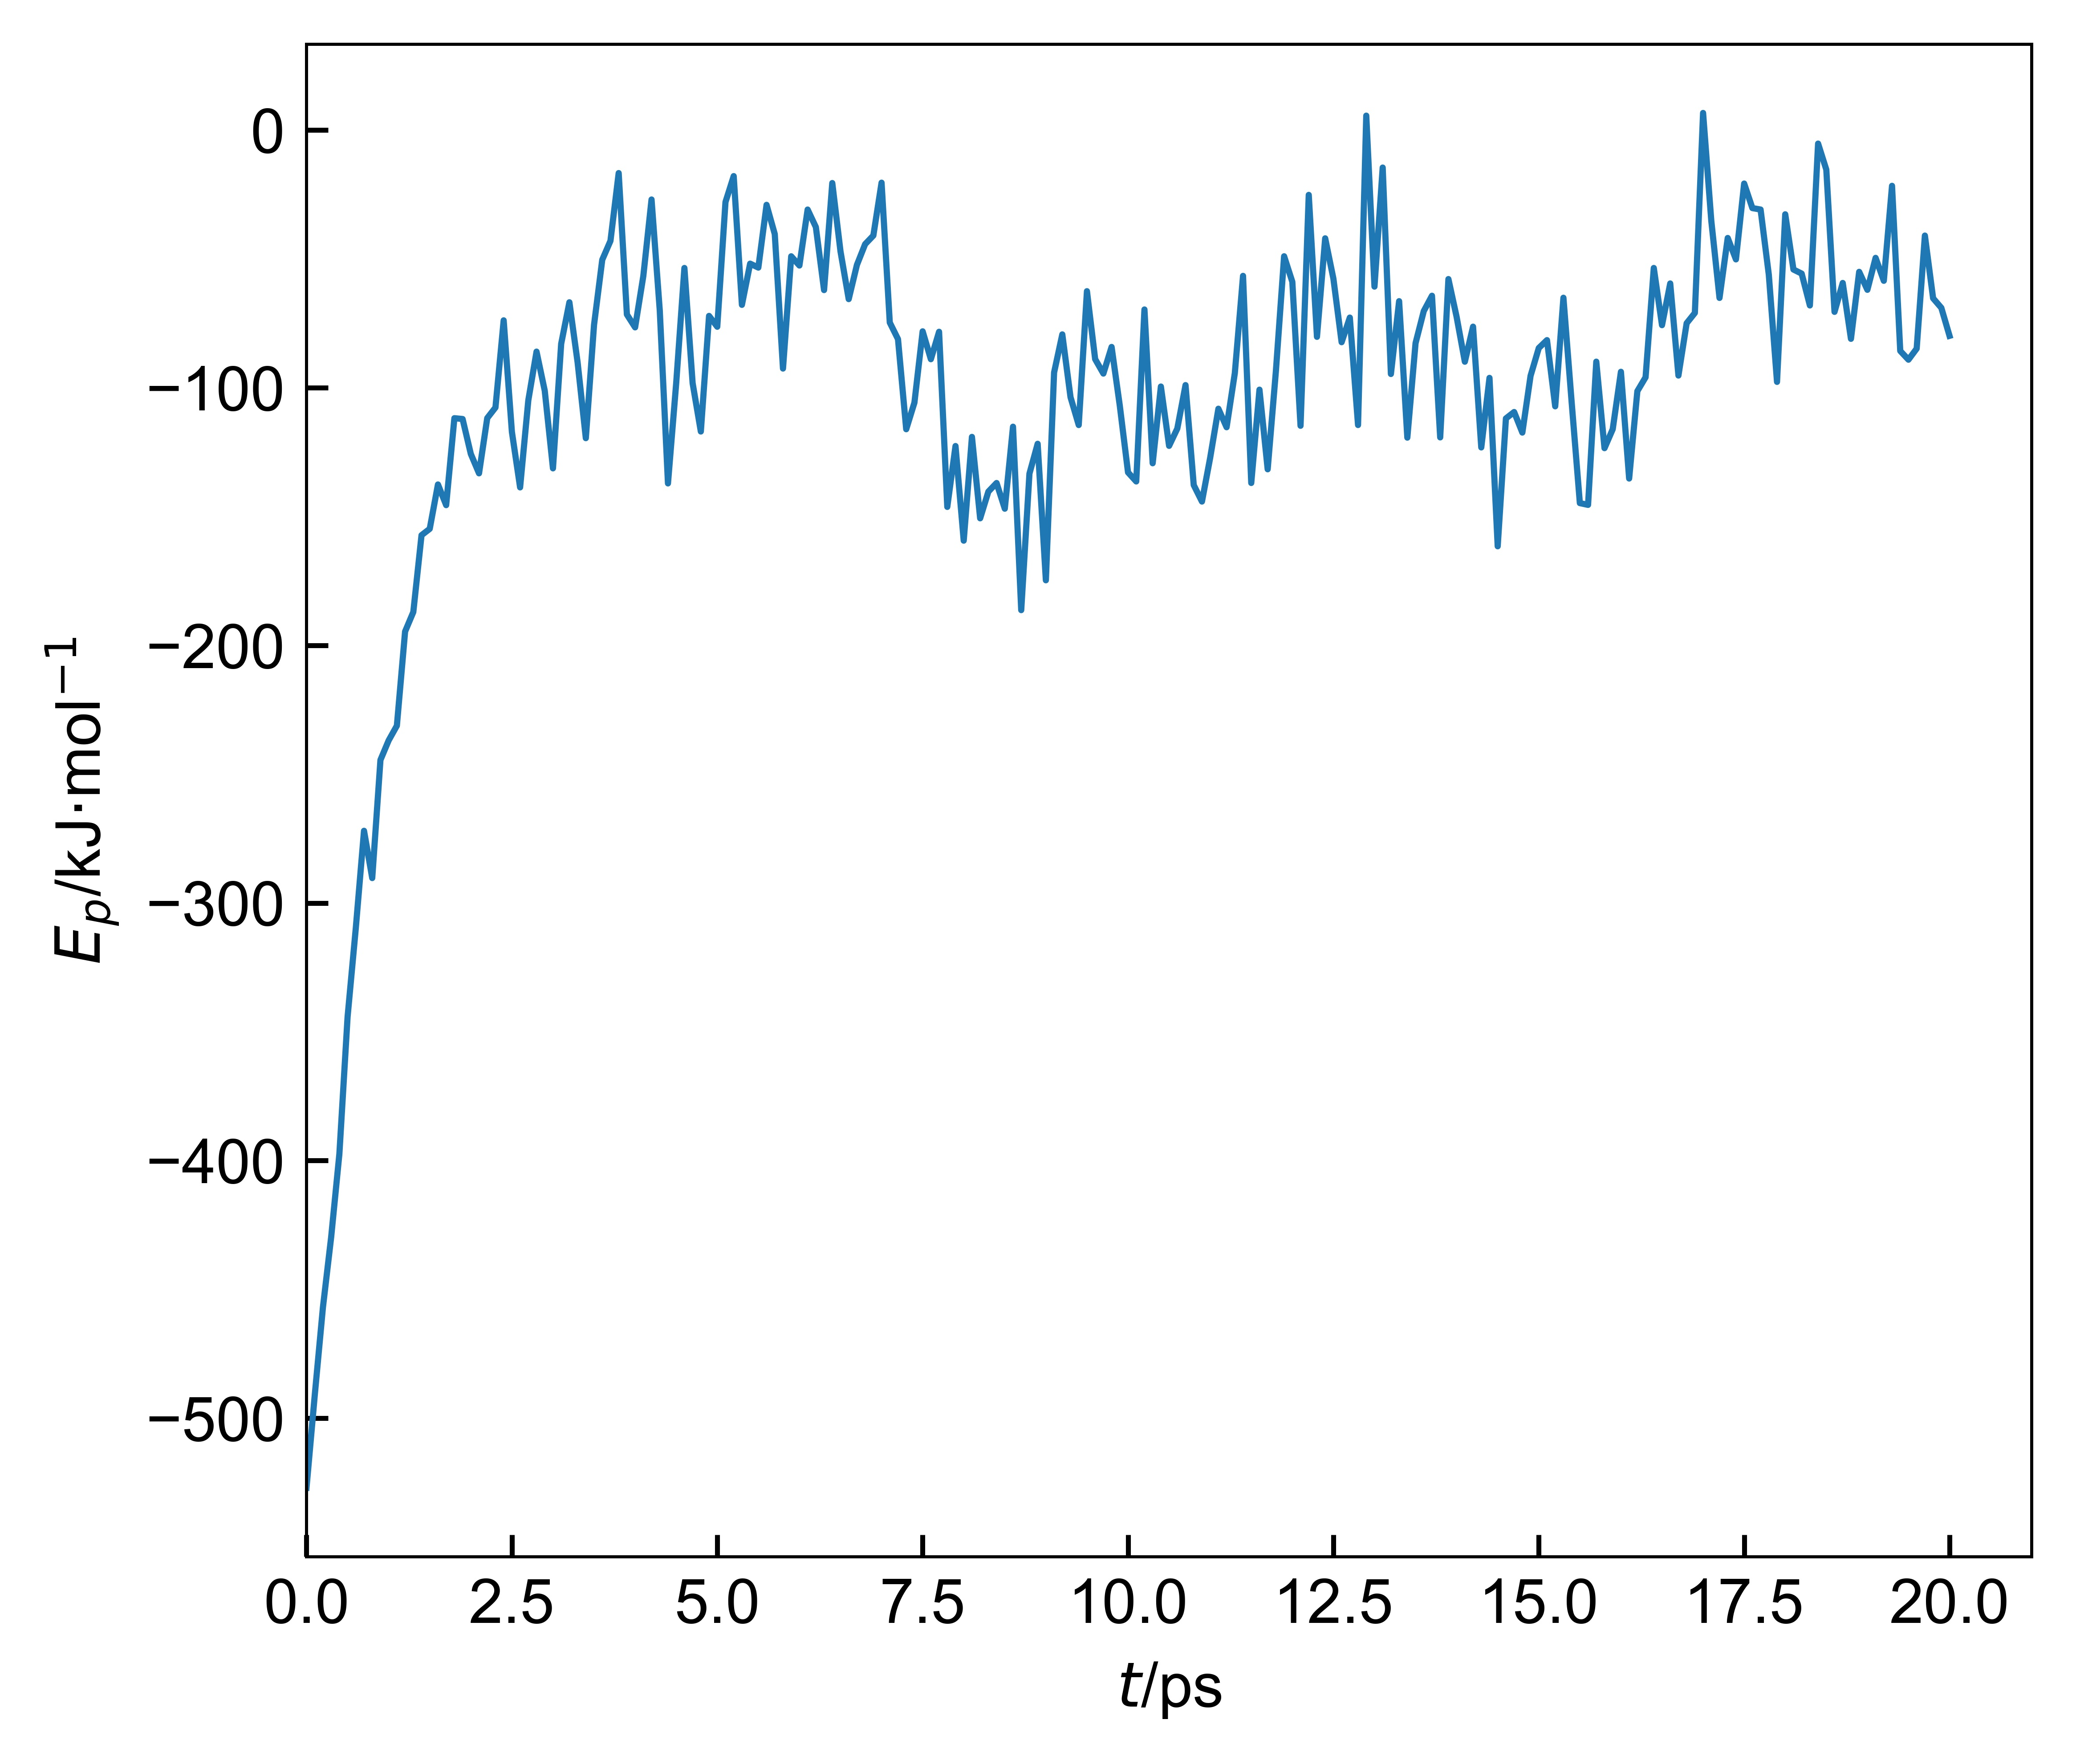
\includegraphics[width=0.5\textwidth]{eptot.jpg}
	\bicaption{丙氨酸12肽链加热升温至300 K体系势能随时间的变化}{System potential energy change of alanine 12 peptide chain heated to 300 K}
\end{figure}
\par

 	\subsubsection{折叠模拟与结果分析}
经过4次折叠模拟,观察到丙氨酸12肽链形成$\alpha$-螺旋;对整个折叠模拟过程的势能按从小到大排序,得到最低势能
$$ E_{pmin}=-74.9130\ \ \rm kcal \cdot mol^{-1} =-313.574\ \ \rm kJ \cdot mol^{-1}$$
对应第4次折叠模拟的539帧;\par
打开VMD程序,载入第4次折叠模拟的轨迹文件ala12\_md4.nc并显示第539帧,在VMD程序可视化窗口中用new cartoon形式显示最低能量结构的构象,如\textbf{图7}所示;
\begin{figure}[h]
	\centering
	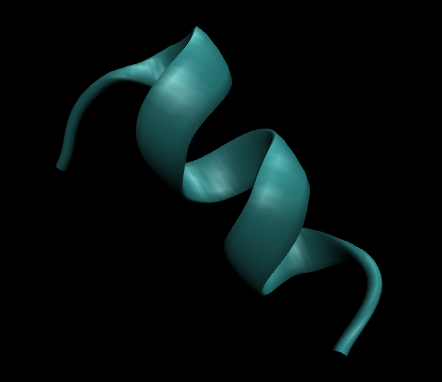
\includegraphics[width=0.45\textwidth]{2.png}
	\bicaption{丙氨酸12肽链折叠模拟过程能量最低构象}{Lowest energy conformation of alanine 12 peptide chain in folding simulation process}
\end{figure}
\par
从\textbf{图7}可以看出,丙氨酸12肽链的最低势能结构形成了较为明显的2圈$\alpha$-螺旋;
读取丙氨酸12肽链4次折叠模拟过程的4个势能文件summary.EPTOT,用python matplotlib包作出整个折叠模拟过程系统势能随时间变化的曲线,如\textbf{图8}所示;从\textbf{图8}可以看出,在整个折叠模拟过程中,系统势能随时间剧烈波动,整体上呈现缓慢下降趋势;系统势能的剧烈波动可能是由于折叠模拟步长过大,导致相邻两帧对应构象的能量有着较大的差别;系统势能整体上缓慢下降,说明在折叠模拟过程中系统具有逐渐演化为能量更低构象的趋势;\par

\begin{figure}[h]
	\centering
	
\includegraphics[width=1.0\textwidth]{ep_md.jpg}
	\bicaption{丙氨酸12肽链折叠模拟过程体系势能随时间的变化}{The change of the potential energy of the system during the folding simulation process}
\end{figure}
需要说明的是,理论上4次折叠模拟总时长为4000 ps,但\textbf{图8}曲线横坐标$t$的最大值显然小于4000 ps;检查各次折叠模拟的输出文件发现,第3次折叠模拟因未知原因提前中止,仅进行了85 ps便在未报错情况下结束,导致折叠模拟的总时长为3185 ps;由于未查阅到相关资料,AMBER 14程序运行过程中也未报错,且只有少数同学出现此类问题,推测是AMBER 14本身的程序bug;对该实验现象的解释有待进一步的研究;\par
读取VMD程序计算得到的折叠模拟过程中与折叠输入的初始构象相比重原子RMSD的结果文件trajrmsd.dat,用python matplotlib包作出整个折叠模拟过程中RMSD随时间变化的曲线,如\textbf{图9}所示;
\begin{figure}[h]
	\centering
	
\includegraphics[width=1.0\textwidth]{rmsd.jpg}
	\bicaption{丙氨酸12肽链折叠模拟过程RMSD随时间的变化}{The change of RMSD of the system during the folding simulation process}
\end{figure}
\par
从\textbf{图9}可以看出,整个折叠模拟过程中,在$0-200\ \ $ps时间段内,RMSD从$0$开始迅速上升,达到第一个峰值;在$200-1400\ \ $ps时间段内,RMSD随时间剧烈波动,并且出现较为明显的峰值,推测原因可能是丙氨酸12肽链结构变化幅度较大,导致RMSD产生剧烈变化;当构象达到峰值时,可能是经历了能量较高的过渡状态;在$1200-3085\ \ $ps时间段内,RMSD随时间的变化较为平稳,推测原因可能是丙氨酸12肽链形成了较为稳定的$\alpha$-螺旋结构,结构变化幅度较小,因此RMSD随时间变化幅度相对较小。
 		
 		

 	
\vbox{}  	
 	 \section{讨论与结论}
		\subsection{实验讨论}
 			\subsubsection{能量最低构象与$\alpha$-螺旋最明显结构不一致的原因分析}
本次实验通过分子动力学模拟方法,利用AMBER 14软件对丙氨酸12肽链进行折叠模拟;在观察折叠模拟过程的轨迹时发现,能量最低构象与$\alpha$-螺旋结构最完整而明显的构象并不完全对应,相反是一个结构相对较“杂乱”的构象,似乎与我们的化学直觉不符,这是否说明分子动力学模拟的方法是不准确的?事实上,对于丙氨酸12肽链而言,其与溶剂的作用也是稳定该分子的重要作用力;在本次实验中我们并未添加溶剂分子,因此可能获得的能量最低构象并不完全准确;随着学习研究的深入,我们可以使用AMBER软件向系统中添加溶剂分子,考虑丙氨酸12肽链分子的溶剂化后,对体系进行更为准确的动力学模拟;另一方面,由于侧链-R基团相互作用等原因,对于丙氨酸12肽链这一分子而言,呈现出最明显$\alpha$-螺旋的结构未必能实际达到能量极小。
 	 	\subsubsection{实验改进}

\par
在折叠模拟过程中,由\textbf{图8}、\textbf{图9}可知,系统势能和RMSD随时间变化较为剧烈,无法得到平滑曲线;这说明每两帧之间系统的构象和能量发生了很大变化,不排除在两帧之间具有更低的能量及其所对应的更优构象;因此,有必要对实验进行一定程度的改进,即适当减小折叠模拟过程的步长,以减小输出的两帧之间分子的构象差异,从而有利于提高计算体系最低势能的精确度和所作势能曲线、RMSD曲线的可读性。
 	 \subsection{实验结论}
本实验通过分子动力学模拟的方法,在Ubuntu系统中运行AMBER 14软件,以丙氨酸12肽链为例,构建了该分子的结构,对初始结构进行了结构优化,对优化后的结构模拟加热升温至300 K,使用VMD软件观察了优化后的结构和加热后的终态构象,记录了加热过程中系统温度、动能、势能的变化;随后对加热后的终态构象进行了4次折叠模拟,观察到了$\alpha$-螺旋的形成,找到了能量最低构象,并记录了折叠模拟过程的系统势能变化和RMSD变化,从而初步了解了分子动力学模拟的基本原理和操作方法,学习了AMBER 14软件的使用;通过分子动力学模拟及VMD软件对经典的$\alpha$-螺旋结构进行了可视化,初步体会了分子动力学模拟的强大威力。
 
 

   

\vbox{}  

\bibliographystyle{achemso}
\bibliography{cite}



\end{document}